%************************************************
\chapter{Introduction}\label{ch:introduction}
%************************************************
The war for talent is on. Coined at the beginning of the new millennium, the term describes the increasing competition between companies for skilled employees\footnote{\url{https://en.wikipedia.org/wiki/The_war_for_talent} | checked June 13, 2015}.

It is on, and it has never been more intense for technical experts\footnote{\url{http://tcrn.ch/1SXBKJl} | checked June 12, 2015}. A perk that one company offers with one job is countered with another perk by another company, and vice versa. Start-up companies are being bought, just for the acquirer to access much needed talent. These so called "aquihires" often lead to an integration of the team into the company and a cancellation of their old product\footnote{\url{http://bit.ly/1FuPbM7} | checked June 13, 2015}\footnote{\url{https://en.wikipedia.org/wiki/Acqui-hiring} | checked June 13, 2015}. It even goes so far that companies bid for talent on online marketplaces, like Hired\footnote{\url{https://hired.com} | checked June 19, 2015} or StartupCV\footnote{\url{https://www.startupcvs.com/} | checked June 19, 2015}.
\newline

Looking at programmers, a candidate for an opening is often put into test projects or given small programming tasks to solve. These should prove programming capability, and - given a successful completion - they are hired\footnote{\url{http://bit.ly/1LDNtvn} | checked June 13, 2015}. Both for developers and recruiters, this process feels slow and tedious, often resulting in frustration for the two. There should be ways of identifying such capabilities beforehand, and rather than conducting technical interviews or costly tests, we propose hereby a software-based method for matching technical talent on to technical requirements from job advertisements.

\section{Contribution}
In this thesis we will present a metric with which developers can be matched against job requirements and be ranked by suitability for it. The metric will build on top of data gathered from analyzed open source repositories. In order to verify it, we also present a platform on which recruiters can easily gain access to these software engineering talents. The recruiters can specify what kind of position they want to find candidates for, and will receive suggestions from the user base that has registered with the application (see figure \ref{fig:employerview}).

GitHub will be the only source of code in our case, but it has proven to be sufficiently large and well-frequented for our use case. The analysis metric has been constructed specifically for our use case, because to the best of our knowledge, no pre-existing method was suitable.

\begin{figure}
  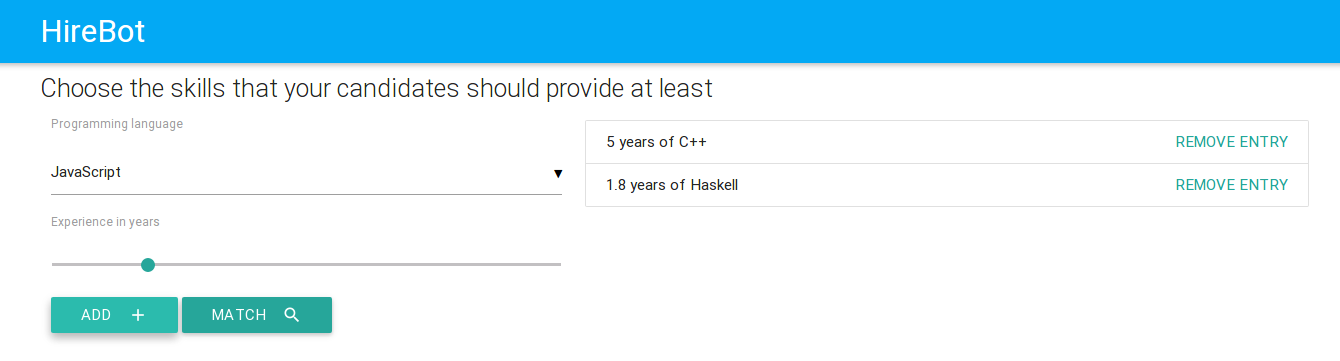
\includegraphics[width=30em]{gfx/employerview.png}
  \caption{The employer search form of Hirebot}
  \label{fig:employerview}
\end{figure}

\section{Research Questions}\label{sec:research-questions}
To guide our research, we formulated two research questions:

\subsection{How can developer skills be measured?}\label{subsec:dev-skill-measurement}
Finding commonalities between job advertisements and skill profiles
requires some sort of reference value. We argue that a measurement
metric needs be found.
In order to reduce the need for a lot of customization
on the advertisements and allow for  analysis of pre-existing data,
it should depend on data provided by most job opening descriptions.
\newline

All developers will be matched against the same job advertisements
and thus they all need to be measured using the same method.
The metric that has been derived from the advertisements will need to be
measured on each developer. Thus the practicability of the metric depends largely on
the availability of measurable data.

\subsection{Can qualified candidates be found automatically?}\label{subsec:measurement-quality}
The metric allows developers to be ranked by suitability for the position. The qualities of this ranking are ultimately determined by whether or not the right candidates land at the top of it. This needs to be verified with real world job candidates and the job opening descriptions that they applied for.

\section{Related Work}

Marlow et al.\cite{md:2013} have conducted an extensive study with about 200 participants, and found out that employers value open source coder profiles greatly.
\marginpar{Marlow et al. have shown that recruiters value open source coder profiles.}
The authors prove that developers are conscious of the fact that their source code is public and thus try to deliver it with great care. This is relevant for us for two reasons: First, it proves that contribution to open source has a relevancy in hiring and is awarded with recognition. And second, the research of Marlow research hints at the fact that developers are trying hard to deliver very good code, because they are aware of its publicity. Because we will use exactly this code in our measurements, it is highly relevant that it be as good as its author can possibly write it. Altogether their research has proven that both public source code repositories are relevant for making recruitment decisions and that open source developers are aware of this fact and try to deliver their best.
\newline

The suitability of source code analysis for the identification of personal skillsets has been demonstrated in the master thesis of Giese\cite{pg:2014}. He built a framework called \textit{Analyzr}\footnote{\url{https://github.com/frontendphil/analyzr}} that analyzes the complete history from a git or SVN source code repository. Based on the code, different metrics are calculated, from which statements about code complexity and refactoring needs can be derived. It is also possible to make statements about developer capabilities and areas of expertise. Thus, given a little context about the analyzed source code, it would possible to say that \glqq Developer X is mainly a backend developer and the single maintainer of module Y\grqq.

Gieses' findings are supported by that of Aftab Iqbal and Michael Hausenblas, who have analyzed different source code repositories for common developers\cite{ih:2012}. They have done so using relatively little local code analysis and relied on on-the-fly analysis from retrieved RDF data. Their work has made it possible to find out whether different open source projects shared developers and contained useful methods of retrieving authors and eliminating duplicates caused by different e-mail addresses, for example. One of their primary sources of code was \textit{sourceforge}, a site that was popular for open source code hosting before GitHub took its place. Now, in 2015, sourceforge has more or less disappeared from the map of open source developers and does not host a lot of projects of relevance anymore.
\newline

Vasilescu et. al. of TU Eindhoven have taken it further and integrated developer-related information across several code forges with crowdsourcing platforms such as StackOverflow\cite{vfs:2012}.
\marginpar{According to Vasilescu, developers are often active on multiple collaborative platforms.}
Their findings allow identifying active contributors on StackOverflow was well as active developers on GitHub.
\newline

A Japanese research group at the Kobe University in Tokyo has displayed great interest in software analytics\cite{mn:2011}. Shinsuke Matsumoto et. al. have built a web service that allowed the analysis of any SVN or git source code repository. They were specifically interested in creating a platform for other researchers to contribute their source code metrics to. The metrics are programming-language agnostic and very general. Unfortunately the code was badly documented and if there was documentation to be found, it was written in Japanese. Matsumotos and Nakamuras paper went into deep technical detail of the inner workings of their platform. This knowledge was particularly helpful in the forming of an architecture for ours. Matsumoto, Nakamura and Giese also hinted at several code metrics of historical importance. They made use of McCabes Cyclomatic Complexity metric\cite{mc:1976} and the Halstead complexity measures\cite{h:1977}. The first provides a way for measuring computational complexity, which is something that might hint at a clean design and a performant implementation. Quite similarly, the latter focuses itself on static code as well, but with the distinction of providing several metrics, like the presumable number of bugs and a code difficulty indicator, all based on four small code-related numbers.
\newline

Algorithmically identifying talent is something that has been tried by many companies with recruiting at the heart of their business model. For LinkedIn, the tools for recruiters that are fueled by this research are their main source of income\footnote{\url{http://tnw.co/1g20G4m} | checked June 29, 2015}. A startup called \textit{Work For Pie}\footnote{\url{http://www.workforpie.com/} | checked June 27, 2015} built a platform similar to ours and got acquired by the hiring platform GroupTalent. For this reason it was very hard to find information on the inner workings of the job recommendation system in production, which is why there is no comparison with their recommendation techniques in this thesis.

\section{Topical background}
The basic concept of applying demand-based filtering can be traced back to a bachelor project at the Hasso-Plattner-Institute.

\marginpar{The bachelor project is a two-semester project at HPI, where 2-7 students work together on a large software system, often for an external partner. In the process, expertise for the bachelor thesis is gathered.}

In a world where cold calls have become outdated\cite{bh:2014}, social media platforms like Facebook, Twitter, LinkedIn and Xing have grown to be important places for getting in touch with customers. 500 million tweets are sent on a single day on Twitter\footnote{\url{https://about.twitter.com/company} | checked June 29, 2015} alone. All platforms combined result in a huge marketing reach. To help covering most of this reach, the bachelor project implemented a system acquiring social media data, applying filtering to it and delivering the sales-relevant pieces via a clean interface.

This eliminates a huge caveat that sales representatives have been facing with social media: Trying to find the \textit{right} information inside this flood of data, which is often referred to as noise. Tiresome during free time and even more stressful if it has to be done on the job. Finding pieces of information which might hint at an interest in a product are the ones sought after daily by sales representatives. Such a finding often leads to an attempt at contacting the author of the entry in question. The information that hints at a consumer interest is commonly referred to as Opportunity.
\newline


The general principle of converting noise to opportunity and reducing information load by applying demand-based-filtering can also be tailored to fit recruiting processes.

\marginpar{Converting noise to opportunity is the very tiring, repetitive task of finding useful information in a heap of thematically but not practically relevant data}

Recruiting may even be mapped roughly on to the problem of selling  products. The \textit{products} are the job vacancies in this case, whereas the \textit{customers} are the potential employees that need to be found. As shown before, there is a heavy competition among recruiters for excellent technical candidates because of their scarcity and it seems a reasonable thought to gain a competitive edge by pre-analyzing technical candidates before considering them for an interview. Also, it makes sense to apply some sort of metric for measuring skill, because
"You can't manage what you can't measure"\cite{tdm:1986}.  People-based metrics need to be seen skeptically, but hiring is such an important decision that it should be manifested with numbers, because it can severely affect company success\cite{hk:1998}.